\section{Remote Client}
\label{sec:rc}
%
The \gls{mdo-rc} is a Desktop application that is developed in QT.
This application handles all the job that is referred to interaction between this last and a \textbf{brand} - to rent an ad or see its statistics - or an \textbf{admin} - to manage all users, stations and ads.

\subsection{Classes}
\label{sub-sec:classes}
%
For a more easier developing, the layout and implementation of this application was divided by 3 distinct \texttt{QWidget} classes:
\begin{enum-c}
\item \texttt{MainWindow} class -- to handle the login and register use cases;
\item \texttt{BrandWindow} class -- to handle everything related to the brand usage;
\item \texttt{AdminWindow} class -- to handle everything related to the admin usage;
\end{enum-c}

\subsubsection{MainWindow class}
%
The \texttt{MainWindow} class is, as it suggests, the main class of all the program.
This class handles all the transitions between views, such as \emph{Login View}, \emph{Admin View}, \emph{Brand View} and \emph{Register View}.

As it can be seen in the header file of this class (listing \ref{lst:mainwindow-h}), there are two pointers to the other two classes, each one of them as a pointer, in order to be instantiated right on the constructor.
The \texttt{Sess *sess} that refers to the \textbf{MySQL session}, the variables associated with threads and the timer will be explaine later on the next section, as well as some functions like thread functions.
%
\lstinputlisting[language=c++, caption={Declaration of MainWindow class},label=lst:mainwindow-h,
style=customc]{./listing/rc-mainwindow.h}%

All the function with the prefix \texttt{"on\_"} on it are private slots that are created to response to the click of some buttons.

Now, looking at the implementation of the Constructor:

\lstinputlisting[language=c++, firstline=25, lastline = 102, caption={Implementation of the constructor \texttt{MainWindow}},label=lst:mainwindow-imp,
style=customc]{./listing/rc-mainwindow.cpp}%

As it can be seen in Listing \ref{lst:mainwindow-imp}, there's an enumerator that helps the class to navigate through the views.
That's because that management is made with the help of \texttt{Stacked Widgets}.
The \textbf{Main Window} also has a pointer to a stacked widget in order to switch between classes and show different views.

In resume, the main steps to have in considering for the \textbf{Remote Client} part are:
\begin{item-c}
\item Initialization of the session to connect to MySQL server;
\item Instantiation of the other two classes;
\item Signals connections to return back to the Main Window after a logout in each class. 
\end{item-c}

\paragraph{\emph{Layout}}
Fig.~\ref{fig:mw-login-view} and fig.~\ref{fig:mw-register-view} show respectively the Login and Register Views.

These two views interact with help of the database. 
For example, when registering a user, if every parameter is correctly inserted, it will be queued a message to MySQL inserting a new User with \textbf{default brand privilege}.
For the example of logging in, it will be made a queue to the MySQL server asking for a row that matches de inputted username and password and if so, the user will be redirectioned to the specific view according to its privileges.

\begin{figure}[htb!]
  \centering
  %
  \begin{subfigure}{.6\textwidth}
  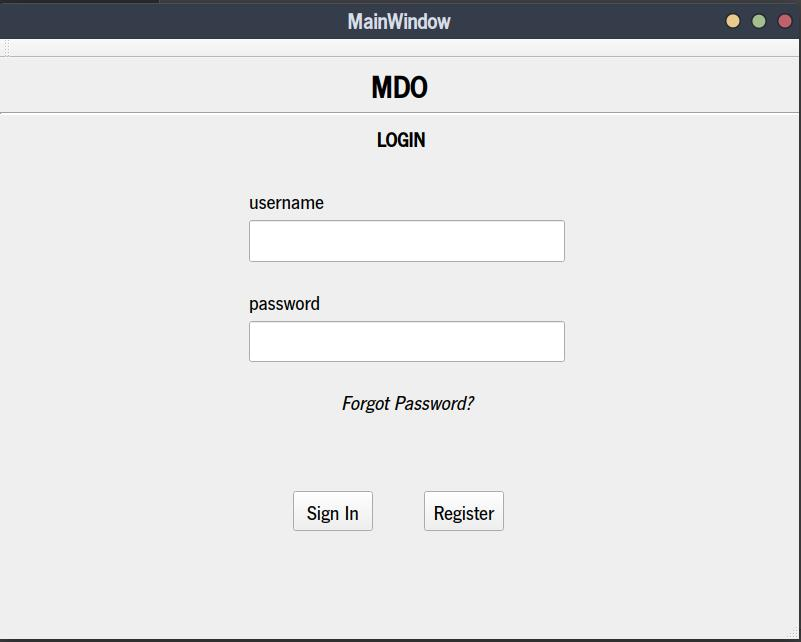
\includegraphics[width=\textwidth]{img/mw-login-view.jpg}%
  \caption{Login View}%
  \label{fig:mw-login-view}
\end{subfigure}

%\hspace{.1\textwidth}
%
  \begin{subfigure}{.6\textwidth}
    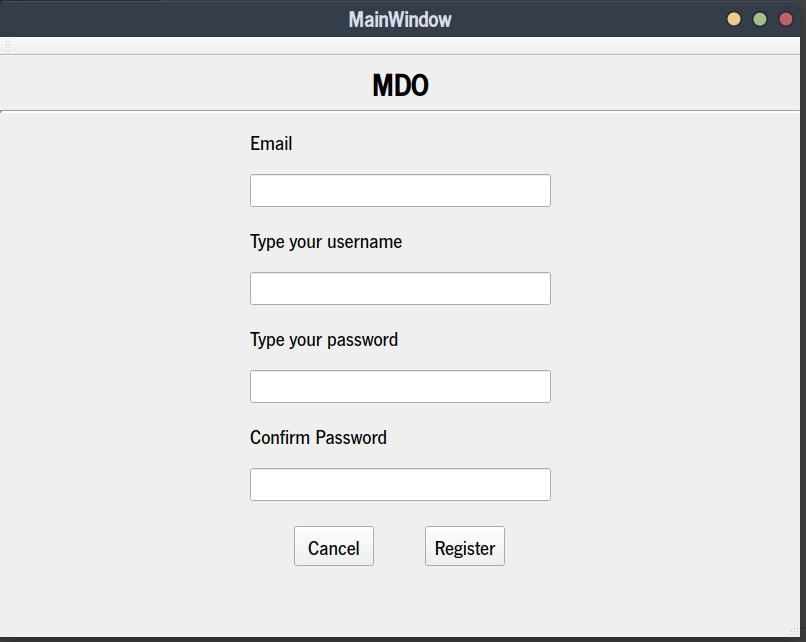
\includegraphics[width=\textwidth]{img/mw-register-view.jpg}%
  \caption{Register View}%
  \label{fig:mw-register-view}
  \end{subfigure}
  % 
  \caption{MainWindow views}%
  \label{fig:ptp-test}
\end{figure}  

\subsubsection{BrandWindow class}
%
The \texttt{BrandWindow} class is, as it suggests, the class that handles all of the brand's features.
This class handles all the transitions between views, such as \emph{Rent Ad View}, \emph{To Rent View} and \emph{Logout} - emits a signal to go back to login.
%
\lstinputlisting[language=c++, caption={Declaration of BrandWindow class},label=lst:brandwindow.h,
style=customc]{./listing/rc-brandwindow.h}%

As it can be seen in the header file of this class (listing \ref{lst:brandwindow.h}), there's also the session to handle the MySQL server connection (\texttt{Sess* sess}), a \texttt{QFileInfo} to handle the files to upload on an Ad and the \texttt{user\_id} which refers to the user that is currently using the app.
As in every part of the code, here there's also the usage of queues to the MySQL server, to rent ads and to see the ads rented to watch its statistics.
In order to make everything more simpler, in the \texttt{Rent View} it is only possible to rent for a range of one week. All the time slots that are already rented appear with a "Rented" \texttt{std::string} and the days that do not correspond to the time space available to rent appear with the label "Unavailable".

Perhaps, one of the most difficult functions to implement was the rent function, that's because it is necessary to add many rows to different tables in order to build a complete Ad on the database, this means that if something went wrong in the middle of the execution, it is necessary to do the inverse process to delete the already inserted rows, because they will not have a link to every tables.

Listing \ref{lst:rent-ad} shows the rent ad function.
%
\lstinputlisting[language=c++, firstline = 341, lastline=462, caption={Implementation of rent function on BrandWindow class},label=lst:rent-ad,
style=customc]{./listing/rc-brandwindow.cpp}

Because of the length and process capability of this function, every little mistake can take to serious consequences, so, it is mandatory to make all and every validation in order to avoid every mistake in the MySQL queue messages. Common errors can be such like redundant blocs of data, or even just a single piece of data.

\paragraph{\emph{Layout}}

Figures \ref{fig:brand-main-view}, \ref{fig:brand-to-rent-view} and \ref{fig:brand-rented-view} show the layout used for all the Brand Views.

\begin{figure}[htb!]
  \centering
  %
  \begin{subfigure}{.4\textwidth}
  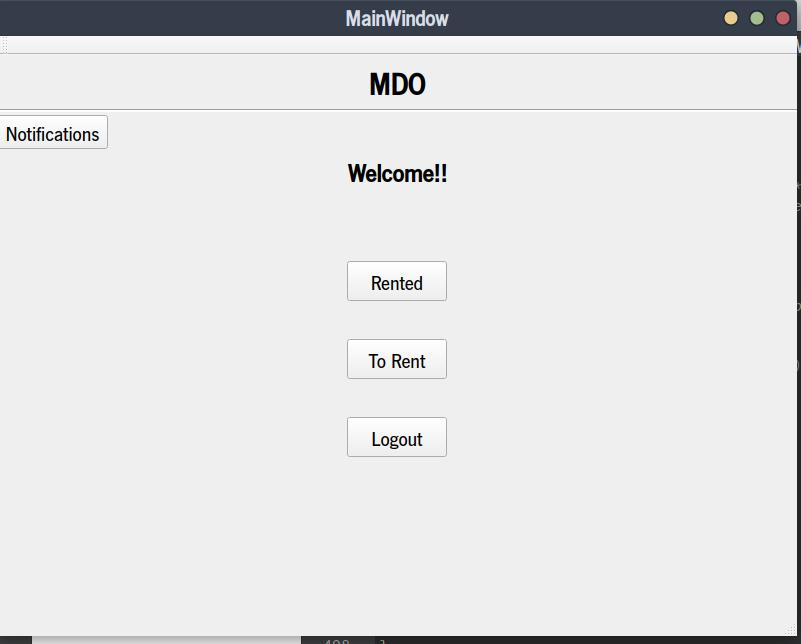
\includegraphics[width=\textwidth]{img/brand-main-view.jpg}%
  \caption{Brand Main View}%
  \label{fig:brand-main-view}
\end{subfigure}

%\hspace{.1\textwidth}
%
  \begin{subfigure}{.4\textwidth}
    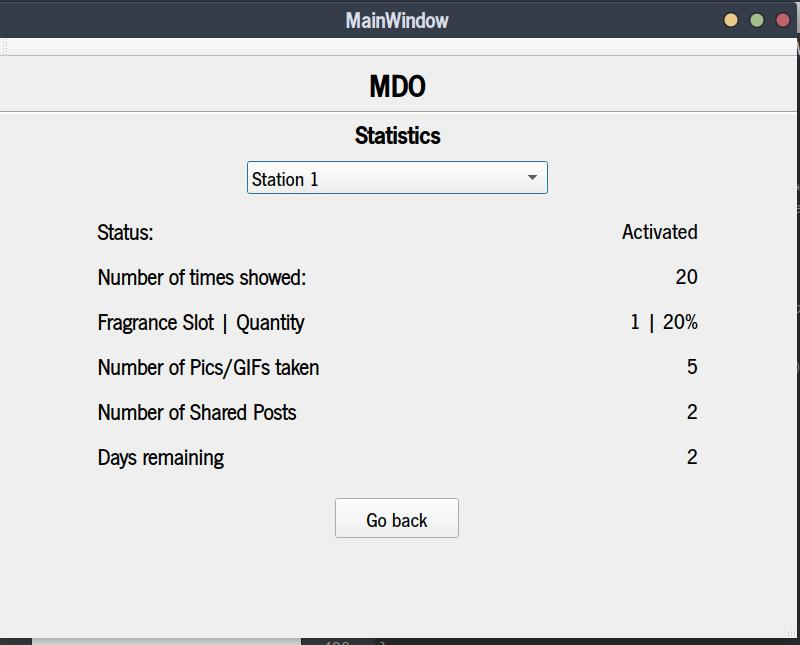
\includegraphics[width=\textwidth]{img/brand-rented-view.jpg}%
  \caption{Brand Rented View}%
  \label{fig:brand-rented-view}
  \end{subfigure}
  % 
  \begin{subfigure}{.4\textwidth}
    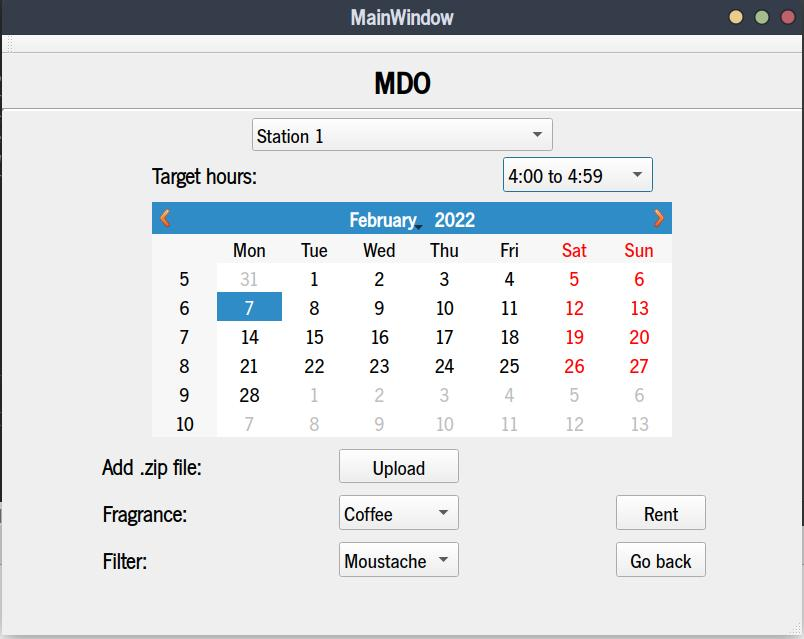
\includegraphics[width=\textwidth]{img/brand-to-rent-view.jpg}%
  \caption{Brand To Rent View}%
  \label{fig:brand-to-rent-view}
  \end{subfigure}
  % 
  \caption{BrandWindow views}%
  \label{fig:ptp-test}
\end{figure} 

\subsubsection{AdminWindow class}
%
The \texttt{AdmindWindow} class is, as it suggests, the class that handles all of the admin's features.
This class handles all the transitions between views, such as \emph{Statistics View}, \emph{Manage Users View}, \emph{Ads To Activate View} and \emph{Test Operation View}.
%
\lstinputlisting[language=c++, caption={Declaration of AdminWindow class},label=lst:adminwindow.h,
style=customc]{./listing/rc-adminwindow.h}%

In terms of private attributes, this class is similar to the \texttt{BrandWindow} class: it has a \texttt{Sess *sess} to handle the communication to MySQL server and it also has a \texttt{user\_id} to know which user is using the app.

Unfortunately, in this case it could not be implemented the Test Operation View because of reasons that will be explained in the next section.

As always, there's a lot of message queues to MySQL in order to handle all the data and shoe them in the \gls{mdo-rc}.
The most interesting feature in this class is the \textbf{Manage Users} function. In this view it is possible to change the permissions of a user, turning into an Admin or a Brand in just a click. It is also possible to delete users, which can be helpful to delete some bots or even users with bad conduct.
Also, the \textbf{Ads to Activate} is an interesting feature, because it can turn ads into active mode or, if denied, it can remove them. This feature is important once it is important to validate all data that is going to be sent to the machines, in order to avoid some type of non-advertisement videos that could appear in the stations.

Listing \ref{lst:admin-manage-users} shows the function \textbf{Manage Users}.
%
\lstinputlisting[language=c++, firstline=273, lastline=306, caption={Implementation of Manage Users from AdminWindow class},label=lst:admin-manage-users,
style=customc]{./listing/rc-adminwindow.cpp}%

Listing \ref{lst:admin-ads-to-act} shows the \textbf{Ads to Activate} feature.
%
\lstinputlisting[language=c++, firstline=376, lastline=430, caption={Implementation of Ads TO Activate from AdminWindow class},label=lst:admin-ads-to-act,
style=customc]{./listing/rc-adminwindow.cpp}%

\paragraph{\emph{Layout}}
%
On figures \ref{fig:admin-main-view}, \ref{fig:admin-manage-users-view} and \ref{fig:admin-ads-to-act-view} are all the views from the Admin Views.

\begin{figure}[htb!]
  \centering
  %
  \begin{subfigure}{.4\textwidth}
  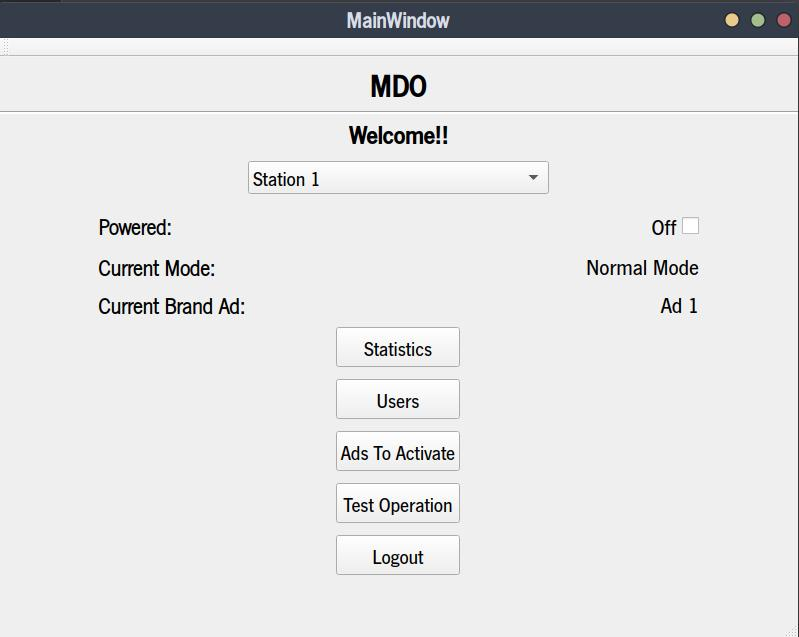
\includegraphics[width=\textwidth]{img/admin-main-view.jpg}%
  \caption{Admin Main View}%
  \label{fig:admin-main-view}
\end{subfigure}

%\hspace{.1\textwidth}
%
  \begin{subfigure}{.4\textwidth}
    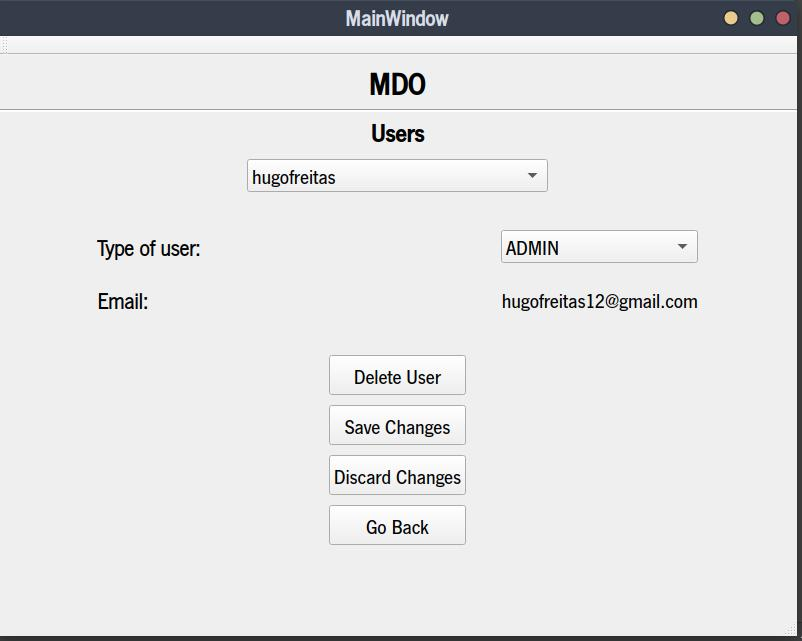
\includegraphics[width=\textwidth]{img/admin-manage-users-view.jpg}%
  \caption{Manage Users View}%
  \label{fig:admin-manage-users-view}
  \end{subfigure}
  % 
  \begin{subfigure}{.4\textwidth}
    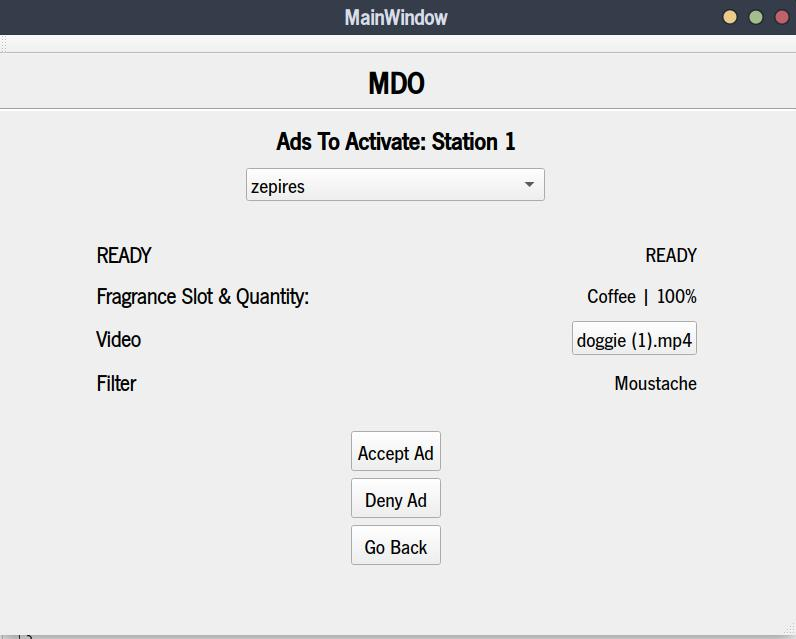
\includegraphics[width=\textwidth]{img/admin-ads-to-act.jpg}%
  \caption{Ads To Activate View}%
  \label{fig:admin-ads-to-act-view}
  \end{subfigure}
  % 
  \caption{AdminWindow views}%
  \label{fig:ptp-test}
\end{figure} 